\documentclass{beamer}
\mode<presentation>{
  \usetheme{Boadilla}
  \usefonttheme[onlylarge]{structurebold}
  \usefonttheme[stillsansseriflarge]{serif}
  \setbeamerfont*{frametitle}{size=\normalsize,series=\bfseries}
  % \setbeamertemplate{navigation symbols}{}
  \setbeamercovered{transparent}
}
\usepackage[english]{babel}
\usepackage[latin1]{inputenc}
\usepackage{times}
\usepackage[T1]{fontenc}
\usepackage{amsmath}
\usepackage{amssymb}
\usepackage{esint}
\usepackage{hyperref}
\usepackage{tikz}
\usepackage{xkeyval}
\usepackage{xargs}
\usepackage{verbatim}
\usepackage{listings}
\usetikzlibrary{
  arrows,
  calc,
  decorations.pathmorphing,
  decorations.pathreplacing,
  decorations.markings,
  fadings,
  positioning,
  shapes
}

\mode<handout>{
  \usepackage{pgfpages}
  \pgfpagesuselayout{4 on 1}[a4paper,landscape,border shrink=5mm]
  \setbeamercolor{background canvas}{bg=black!10}
}

\newcommand\pgfmathsinandcos[3]{%
  \pgfmathsetmacro#1{sin(#3)}%
  \pgfmathsetmacro#2{cos(#3)}%
}
\newcommand\LongitudePlane[3][current plane]{%
  \pgfmathsinandcos\sinEl\cosEl{#2} % elevation
  \pgfmathsinandcos\sint\cost{#3} % azimuth
  \tikzset{#1/.estyle={cm={\cost,\sint*\sinEl,0,\cosEl,(0,0)}}}
}
\newcommand\LatitudePlane[3][current plane]{%
  \pgfmathsinandcos\sinEl\cosEl{#2} % elevation
  \pgfmathsinandcos\sint\cost{#3} % latitude
  \pgfmathsetmacro\yshift{\cosEl*\sint}
  \tikzset{#1/.estyle={cm={\cost,0,0,\cost*\sinEl,(0,\yshift)}}} %
}
\newcommand\DrawLongitudeCircle[2][1]{
  \LongitudePlane{\angEl}{#2}
  \tikzset{current plane/.prefix style={scale=#1}}
  % angle of "visibility"
  \pgfmathsetmacro\angVis{atan(sin(#2)*cos(\angEl)/sin(\angEl))} %
  \draw[current plane] (\angVis:1) arc (\angVis:\angVis+180:1);
  \draw[current plane,dashed] (\angVis-180:1) arc (\angVis-180:\angVis:1);
}
\newcommand\DrawLatitudeCircleArrow[2][1]{
  \LatitudePlane{\angEl}{#2}
  \tikzset{current plane/.prefix style={scale=#1}}
  \pgfmathsetmacro\sinVis{sin(#2)/cos(#2)*sin(\angEl)/cos(\angEl)}
  % angle of "visibility"
  \pgfmathsetmacro\angVis{asin(min(1,max(\sinVis,-1)))}
  \draw[current plane,decoration={markings, mark=at position 0.6 with {\arrow{<}}},postaction={decorate},line width=.6mm] (\angVis:1) arc (\angVis:-\angVis-180:1);
  \draw[current plane,dashed,line width=.6mm] (180-\angVis:1) arc (180-\angVis:\angVis:1);
}
\newcommand\DrawLatitudeCircle[2][1]{
  \LatitudePlane{\angEl}{#2}
  \tikzset{current plane/.prefix style={scale=#1}}
  \pgfmathsetmacro\sinVis{sin(#2)/cos(#2)*sin(\angEl)/cos(\angEl)}
  % angle of "visibility"
  \pgfmathsetmacro\angVis{asin(min(1,max(\sinVis,-1)))}
  \draw[current plane] (\angVis:1) arc (\angVis:-\angVis-180:1);
  \draw[current plane,dashed] (180-\angVis:1) arc (180-\angVis:\angVis:1);
}
\newcommand\coil[1]{
  {\rh * cos(\t * pi r)}, {\apart * (2 * #1 + \t) + \rv * sin(\t * pi r)}
}
\makeatletter
\define@key{DrawFromCenter}{style}[{->}]{
  \tikzset{DrawFromCenterPlane/.style={#1}}
}
\define@key{DrawFromCenter}{r}[1]{
  \def\@R{#1}
}
\define@key{DrawFromCenter}{center}[(0, 0)]{
  \def\@Center{#1}
}
\define@key{DrawFromCenter}{theta}[0]{
  \def\@Theta{#1}
}
\define@key{DrawFromCenter}{phi}[0]{
  \def\@Phi{#1}
}
\presetkeys{DrawFromCenter}{style, r, center, theta, phi}{}
\newcommand*\DrawFromCenter[1][]{
  \setkeys{DrawFromCenter}{#1}{
    \pgfmathsinandcos\sint\cost{\@Theta}
    \pgfmathsinandcos\sinp\cosp{\@Phi}
    \pgfmathsinandcos\sinA\cosA{\angEl}
    \pgfmathsetmacro\DX{\@R*\cost*\cosp}
    \pgfmathsetmacro\DY{\@R*(\cost*\sinp*\sinA+\sint*\cosA)}
    \draw[DrawFromCenterPlane] \@Center -- ++(\DX, \DY);
  }
}
\newcommand*\DrawFromCenterText[2][]{
  \setkeys{DrawFromCenter}{#1}{
    \pgfmathsinandcos\sint\cost{\@Theta}
    \pgfmathsinandcos\sinp\cosp{\@Phi}
    \pgfmathsinandcos\sinA\cosA{\angEl}
    \pgfmathsetmacro\DX{\@R*\cost*\cosp}
    \pgfmathsetmacro\DY{\@R*(\cost*\sinp*\sinA+\sint*\cosA)}
    \draw[DrawFromCenterPlane] \@Center -- ++(\DX, \DY) node {#2};
  }
}
\makeatother

% not mandatory, but I though it was better to set it blank
\setbeamertemplate{headline}{}
\def\beamer@entrycode{\vspace{-\headheight}}

\tikzstyle{snakearrow} = [decorate, decoration={pre length=0.2cm,
  post length=0.2cm, snake, amplitude=.4mm,
  segment length=2mm},thick, ->]

%% document-wide tikz options and styles

\tikzset{%
  % >=latex, % option for nice arrows
  inner sep=0pt,%
  outer sep=2pt,%
  mark coordinate/.style={inner sep=0pt,outer sep=0pt,minimum size=3pt,
    fill=black,circle}%
}
\tikzset{
  % Define standard arrow tip
  >=stealth',
  % Define style for boxes
  punkt/.style={
    rectangle,
    rounded corners,
    draw=black, very thick,
    text width=8em,
    minimum height=2.5em,
    text centered},
}
\makeatletter
\newbox\@backgroundblock
\newenvironment{backgroundblock}[2]{%
  \global\setbox\@backgroundblock=\vbox\bgroup%
  \unvbox\@backgroundblock%
  \vbox to0pt\bgroup\vskip#2\hbox to0pt\bgroup\hskip#1\relax%
}{\egroup\egroup\egroup}
\addtobeamertemplate{background}{\box\@backgroundblock}{}
\makeatother

% \def\timeleft{15:00->14:55}

\title[Computer control]{Computer control of the \textbf{NaCs} experiment}
\author{Yichao Yu}
\institute{Ni Group/Harvard}

\begin{document}

\begin{frame}{}
  \titlepage
\end{frame}

% Intro
% \def\timeleft{14:55->14:20}
\begin{frame}{}
  \begin{block}{Without precise timing}
    \begin{itemize}[<+->]
    \item
      Vapor pressure
    \item
      MOT loading
    \item
      Objective alignment
    \end{itemize}
  \end{block}
  \begin{block}{Measurements that require precise timing}
    \begin{itemize}[<+->]
    \item
      Polarization gradient cooling
    \item
      Temperature calibration
    \item
      ODT loading
    \item
      $\cdots\cdots\cdots$
    \end{itemize}
  \end{block}
\end{frame}

% \def\timeleft{14:20->13:50}
\begin{frame}{}
  \tableofcontents
\end{frame}

% \def\timeleft{13:50->11:40}
\section{Hardware}
\begin{frame}{Hardware}
  \only<+->{
    \begin{backgroundblock}{0pt}{0pt}
      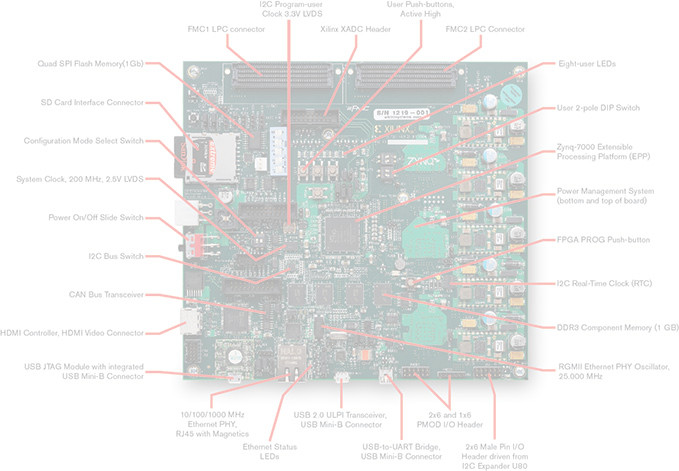
\includegraphics[width=\paperwidth]{zc702-baseboard_sm_bg.jpg}
    \end{backgroundblock}
  }
  \only<1-2>{
    \begin{backgroundblock}{0pt}{0pt}
      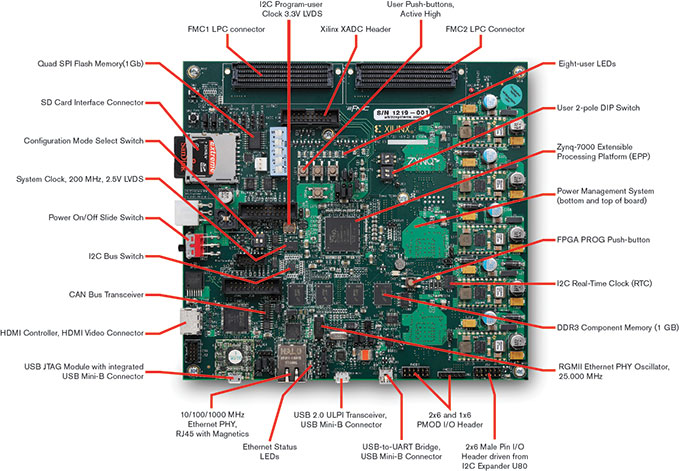
\includegraphics[width=\paperwidth]{zc702-baseboard_sm.jpg}
    \end{backgroundblock}
  }
  \only<3>{
    \begin{backgroundblock}{0pt}{0pt}
      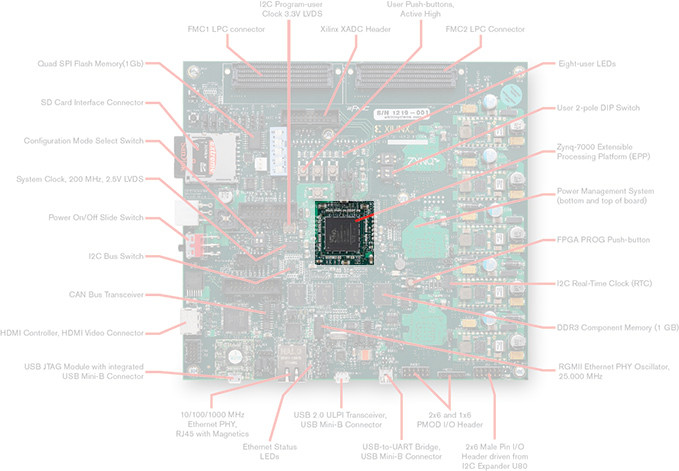
\includegraphics[width=\paperwidth]{cpu.jpg}
    \end{backgroundblock}
  }
  \only<4>{
    \begin{backgroundblock}{0pt}{0pt}
      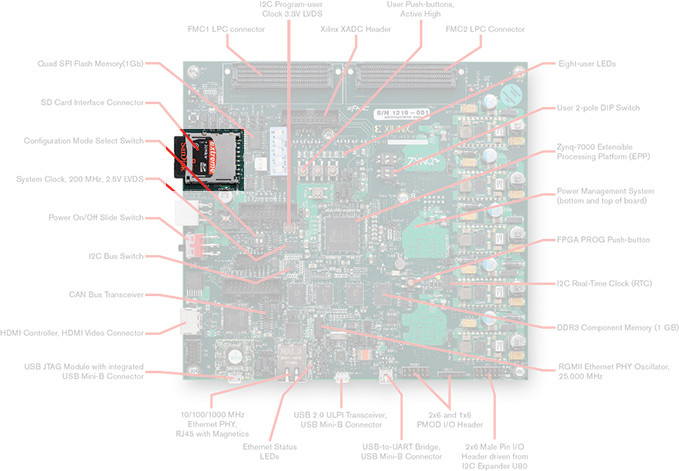
\includegraphics[width=\paperwidth]{sd_card.jpg}
    \end{backgroundblock}
  }
  \only<5>{
    \begin{backgroundblock}{0pt}{0pt}
      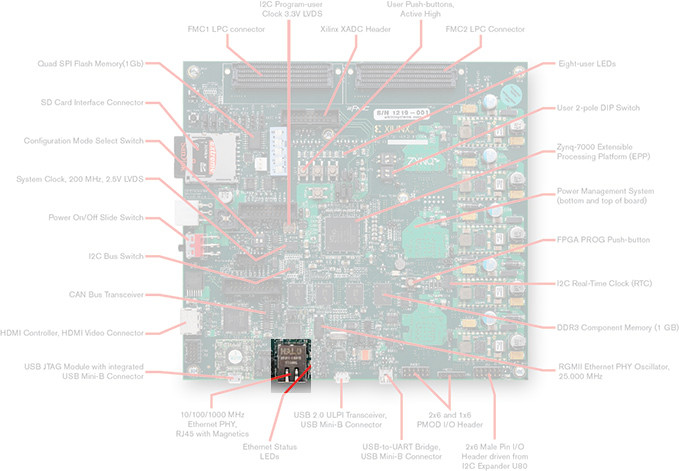
\includegraphics[width=\paperwidth]{ethernet.jpg}
    \end{backgroundblock}
  }
  \only<6>{
    \begin{backgroundblock}{0pt}{0pt}
      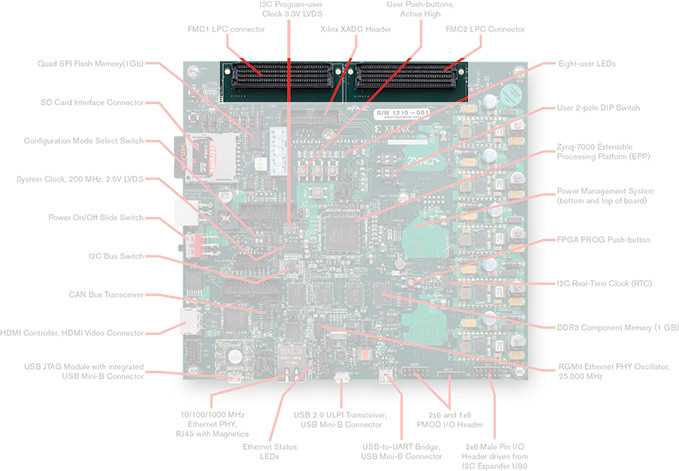
\includegraphics[width=\paperwidth]{fmc.jpg}
    \end{backgroundblock}
  }
  \begin{columns}
    \column{5.5cm}
    \only<7->{
      \begin{block}{Output}
        \begin{itemize}
        \item
          TTL $\times 24$
        \item<8->
          DDS $\times 22$
        \item<9->
          DAC from NI PCIe card (WIP)
        \end{itemize}
      \end{block}
    }
    \column{5.5cm}
    \only<+->{
      \vspace{4cm}
      \begin{block}{FPGA mother board}
        \begin{itemize}
        \item
          ZC702 Evaluation Kit
        \item<+->
          FPGA + Dual core ARM CPU
        \item<+->
          SD Card
        \item<+->
          1Gb Ethernet
        \item<+->
          FMC extension connectors
        \end{itemize}
      \end{block}
    }
  \end{columns}
\end{frame}

\section{MOT temperature}
\begin{frame}{}
  \begin{columns}
    \column{7cm}
    \only<+->{}
    \only<-5>{
      \tiny
      \lstinputlisting[language=Python, lastline=32]{mot.txt}
    }
    \only<6-> {
      \begin{block}{Cesium MOT temperature}
        \begin{itemize}
        \item
          $TOF\approx3\text{ms}$
        \item<7->
          $T\approx1\text{mK}$
        \end{itemize}
      \end{block}
    }
    \column{5cm}
    \only<+-> {
      \begin{tikzpicture}[scale=.8]
        \path (0, 2) node (dummy) {};
        \path (0, 0) node[punkt] (mot) {MOT loading};
        \only<+-> {
          \path (0, -2) node[punkt] (release) {Release (Light and field off)};
          \draw[->, thick] (mot) -- (release);
        }
        \only<+-> {
          \path (0, -4) node[punkt] (tof) {Wait (TOF)};
          \draw[->, thick] (release) -- (tof);
        }
        \only<+-> {
          \path (0, -6) node[punkt] (image) {Image (Light on)};
          \draw[->, thick] (tof) -- (image);
        }
        \path (0, -8) node (dummy) {};
      \end{tikzpicture}
    }
  \end{columns}
\end{frame}

\section{Looking for single atom in the ODT}
\begin{frame}{}
\end{frame}

\end{document}
